\documentclass[a4paper, 12pt]{article}

%%% SST LAB PROTOCOLL PREAMBLE
%%% 2019
%%%%%%%%%%%%%%%%%%%%%%%%%%%%%%%


%%% PACKAGES
%%%%%%%%%%%%%%%%%%%%%%%%%%%

\usepackage[ngerman]{babel}

\usepackage[utf8]{inputenc}
\usepackage{amsmath}
\usepackage{pgfplots}
\usepackage{tikz}
\usepackage[many]{tcolorbox}
\usepackage{graphicx}
\graphicspath{ {./graphics/} }
\usepackage{pdfpages}
\usepackage{dashrule}
\usepackage{float}
\usepackage{siunitx}
\usepackage{trfsigns}
\usepackage{booktabs}
\usepackage[european]{circuitikz}
\usepackage{tcolorbox}

%%% DOCUMENT GEOMETRY
%%%%%%%%%%%%%%%%%%%%%%%%%%%

\usepackage{geometry}
\geometry{
 a4paper,
 total={0.6180339887498948\paperwidth,0.6180339887498948\paperheight},
 top = 0.1458980337503154\paperheight,
 bottom = 0.1458980337503154\paperheight
 }
\setlength{\jot}{0.013155617496424828\paperheight}
\linespread{1.1458980337503154}

\setlength{\parskip}{0.013155617496424828\paperheight} % paragraph spacing


%%% COLORS
%%%%%%%%%%%%%%%%%%%%%%%%%%%

\definecolor{red1}{HTML}{f38181}
\definecolor{yellow1}{HTML}{fce38a}
\definecolor{green1}{HTML}{95e1d3}
\definecolor{blue1}{HTML}{66bfbf}
\definecolor{hsblue}{HTML}{00b1db}
\definecolor{hsgrey}{HTML}{afafaf}

%%% CONSTANTS
%%%%%%%%%%%%%%%%%%%%%%%%%%%
\newlength{\smallvert}
\setlength{\smallvert}{0.0131556\paperheight}


%%% COMMANDS
%%%%%%%%%%%%%%%%%%%%%%%%%%%

% differential d
\newcommand*\dif{\mathop{}\!\mathrm{d}}

% horizontal line
\newcommand{\holine}[1]{
  	\begin{center}
	  	\noindent{\color{hsgrey}\hdashrule[0ex]{#1}{1pt}{3mm}}\\%[0.0131556\paperheight]
  	\end{center}
}

% mini section
\newcommand{\minisec}[1]{ \noindent\underline{\textit {#1} } \\}

% quick function plot
\newcommand{\plotfun}[3]{
  \vspace{0.021286\paperheight}
  \begin{center}
    \begin{tikzpicture}
      \begin{axis}[
        axis x line=center,
        axis y line=center,
        ]
        \addplot[draw=red1][domain=#2:#3]{#1};
      \end{axis}
    \end{tikzpicture}
  \end{center}
}

% box for notes
\newcommand{\notebox}[1]{

\tcbset{colback=white,colframe=green1!100!black,title=Note!,width=0.618\paperwidth,arc=0pt}

 \begin{center}
  \begin{tcolorbox}[]
   #1 
  \end{tcolorbox}
 
 \end{center} 
 
}

% box for equation
\newcommand{\eqbox}[2]{
	
	\tcbset{colback=white,colframe=green1!100!black,title=,width=#2,arc=0pt}
	
	\begin{center}
		\begin{tcolorbox}[ams align*]
				#1
		\end{tcolorbox}
		
	\end{center} 
	
}
% END OF PREAMBLE

%%%%%%%%%%%%%%%%%%%%%%%%%%%%%%%%%%%%%
\begin{document}

%%%%%%%%%%%%%%%%%%%%%%%%%%%%%%%%%%%%%
  
\includepdf{./titlepage/titlepage.pdf}
  \clearpage
  \setcounter{page}{1}
%%%%%%%%%%%%%%%%%%%%%%%%%%%%%%%%%%%%%

\section{Vorbereitungsaufgaben}

  \subsection{Netzwerkanalysator}
   Ein Netzwerkanalysator misst die Netzwerkparameter elektrischer Netzwerke,
insbesondere Vierpoleigenschaften, wie
\begin{itemize}
  \item Impedanz,
  \item Reflexionsfaktor,
  \item Transmission (Übertragungsfunktion),
\end{itemize}
deren Werte als Frequenzgänge auf einem Bildschirm dargestellt werden.

Ein skalarer Netzwerkanalysator (SNA) misst nur die Beträge der entsprechenden
Größen, ein vektorieller Netzwerkanalysator (VNA)
hingegen misst Beträge \textbf{und} Phasen, also \emph{komplexe} Werte (der Begriff
\emph{vektoriell} ist daher etwas irreführend).


  \subsection{Kalibrierung und -standards}
   Bei einer Messung treten gewöhnlicherweise systematische Fehler auf. Diese sind
durch die Messeinrichtung bedingt und müssen vor der Messung erfasst und
korrigiert werden, um möglichst genaue Messergebnisse erzielen zu können. Diese
Störeinflüsse treten z.B. durch die ungewollten Eigenschaften von Messleitungen
auf, da sie eigene Übertragungsfunktionen und Reflexionsfaktoren besitzen,
welche das Messergebnis verfälschen.

Bei der \emph{Kalibrierung} wird die Abweichung der Messeinrichtung mit einem
Referenzobjekt (Standard, Normal) verglichen. Beim Netzwerkanalysator ist dies
typischerweise ein \glqq Short, Open, Load\grqq (SOL) bzw. \glqq Short, Open,
Load, Through\grqq (SOLT), welches die Messleitung (Kabel, Verbindungen) mit den jeweiligen Impedanzen
abschließt (Mech-Cal). Diese werden nacheinander mit den verwendeten Ports des NWAs
verbunden. Die Kalibrierung kann ebenfalls mit einem automatischen
Kalibrierungsmodul (eCal) durchgeführt werden, welches für jeden Port die
entsprechenden Kalibrierungsbedingungen automatisch bereitstellt. Diese Methode
verringert die mechanische Belastung der Verbindungen und ist, gerade bei 4-Port-Kalibrierung, schneller.

Vor der Kalibrierung des NWAs muss der zu messende Frequenzbereich eingestellt
werden (start \& stop frequency). Bei einer Umstellung des Frequenzbereiches muss
erneut kalibriert werden.

  \subsection{Parameter}
  \subsubsection{Einfügedämpfung}
Die Einfügedämpfung ist das Verhältnis der Leistung, die an einer Last über z.B.
eine Leitung umgesetzt wird, zu der Leistung, die
\emph{direkt} an der Last umgesetzt werden würde (ohne die Leitung). Sie gibt
also den Leistungsverlust bzw. die Dämpfung an, die das Signal durch das \textit{Einfügen} der Leitung in den
Signalweg erfährt.

\subsubsection{Verstärkung}
Die Verstärkung ist allgemein das Verhältnis von Ausgangs- zu Eingangsgröße,
also z.B. Aus- zu Eingangsspannung. Ist die Verstärkung kleiner eins, handelt es
sich um eine Dämpfung. Logarithmisch/im Dezibel-Maß kann sie abhängig von der
betrachtetn Größe dargestellt werden durch
\[V = 10 \cdot \log_{10}{\frac{P_2}{P_1}}\]
wenn es sich um eine Leistung handelt oder
\[V = 20 \cdot \log_{10}{\frac{U_2}{U_1}}\]
wenn es sich um eine Spannung handelt.

\subsubsection{Reflexionsdämpfung}
Die Reflexionsdämpfung $R$ ist die Dämpfung der reflektierten Welle.
\[R = \frac{P_\mathrm{reflektiert}}{P_\mathrm{ein}}\]
Sie entspricht dem inversen Reflexionsfaktor.


\subsubsection{S-Parameter}
Die S(treu)-Parameter (vom engl. \emph{Scattering-Parameter}) sind eine Reihe an
komplexwertigen Parametern (Betrag + Phase) zur Charakterisierung von n-Toren,
in der Regel Vierpole.

Bei der Berechnung der S-Parameter bezieht man sich auf ein Vierpolmodell, bei
welchem $a_1$ und $a_2$ die auf das jeweilige Tor zulaufenden und $b_1$ und
$b_2$ die vom jeweiligen Tor ablaufenden Wellengrößen sind (Tor 1/Tor 2).

Bei einem Vierpolnetzwerk existieren die folgenden S-Parameter:
\begin{description}
  \item[$S_{11}$, der Reflexionskoeffizient, primärseitig,] beschreibt das
    Reflexions-zu-Transmissions-Verhältnis von Spannungs- bzw. Stromwellen.
    \[S_{11} = \frac{b_1}{a_1}\]
    \item[$S_{21}$, der Transmissionskoeffizient, primärseitig,] beschreibt das
      Verhältnis der am Tor 2 auslaufenden Welle zur am Tor 1 einlaufenden
      Welle. Über der Frequenz also die Übertragungsfunktion. (\glqq Ausgang zu
      Eingang\grqq)
      \[S_{21} = \frac{b_2}{a_1}\]
    \item[$S_{22}$, der Reflexionskoeffizient, sekundärseitig]
      Wie $S_{11}$ nur vom anderen Tor blickend.
      \[S_{22} = \frac{b_2}{a_2}\]
    \item[$S_{12}$, der Transmissionskoeffizient, sekundärseitig]
      Wie $S_{21}$ nur vom anderen Tor blickend.
      \[S_{12} = \frac{b_1}{a_2}\]
\end{description}

Der erste Index steht jeweils für den Wirkungsort, der zweite für die Ursache.


  \subsection{Elektrische Länge}
  Zur Bestimmung der elektrischen Länge wird die Phasenlage des Signals benötigt.
Mit einem zeitlichen Delay/Korrekturparameter kann dann die Laufzeit bestimmen
(Phasenlage = 0), woraus sich mit dem Verkürzungsfaktor die physikalische Länge berechnen lässt.

  \subsection{Stecker- und Messadapternormen}
  \begin{table}[H]
  \begin{center}
    \begin{tabular}{ll}
      \rowcolor{gray0}
      Typ                         & Frequenzbereich            \\
      BNC                         & $< 4\, \si{\giga\hertz}$   \\
      SMC                         & $< 12 \, \si{\giga\hertz}$ \\
      TNC                         & $< 12 \, \si{\giga\hertz}$ \\
      N(eill)                     & $< 12\, \si{\giga\hertz}$  \\
      SMA                         & $< 18 \, \si{\giga\hertz}$ \\
      C                           & $< 11 \, \si{\giga\hertz}$ \\
      $2.94 \, \si{\milli\meter}$ & $< 40 \, \si{\giga\hertz}$ \\
      $2.4 \, \si{\milli\meter}$  & $< 50\, \si{\giga\hertz}$  \\
      $1.85 \, \si{\milli\meter}$ & $< 67\, \si{\giga\hertz}$  \\
      $1 \, \si{\milli\meter}$    & $< 110\, \si{\giga\hertz}$
    \end{tabular}
\end{center}
\caption{Einige Verbindungstypen und deren Einsatz-Frequenzbereiche}
\end{table}

  \subsection{Verkürzungsfaktor}
  Im freien Raum breiten sich elektromagnetische Wellen mit der Lichgeschwindigkeit
\[c_0 \approx 3 \cdot 10^8\]
aus, welche die maximale Ausbreitungsgeschwindigkeit für Energie und Information
darstellt. In Leitungen ist die Ausbreitungsgeschwindigkeit $c$ von Spannungs- und
Stromwellen jedoch geringer. Dadurch erscheint die Wellenlänge $\lambda$ auf der Leitung
gegenüber der Wellenlänge im Vakuum $\lambda_0$ verkürzt. Das Verhältnis ist der Verkürzungsfaktor.
\[\frac{\lambda}{\lambda_0} = VK\]
Für die Wellenlänge auf der Leitung ergibt sich damit
\[\lambda = \frac{c}{f} = VK \cdot \frac{c_0}{f}\]

Der konkrete Wert des Verkürzungsfaktors ist von der Bauart der Leitung
abhängig. Für eine koaxiale Leitung ergibt sich beispielsweise
\[ {VK} = \frac{1}{\sqrt{\epsilon_r}}\]
Für ein Koaxialkabel mit einem Dielektrikum aus Polyethylen ($\epsilon_r =
2.25$) erhält man somit einen Verkürzungsfaktor von (näherungsweise) $VK = 0.667$.


\section{Versuchsaufgaben}

\subsection{Kalibrierung}
Die menügesteuerte Kalibrierung des Netzwerkanalysators erfolgte in einem Frequenzbereich von
$10 \, \si{\mega\hertz}$ bis $6 \, \si{\giga\hertz}$ mithilfe des elektronischen
Kalibrierungskits an allen vier Ports. 

\subsection{S11-Messung}
\begin{figure}[h]
  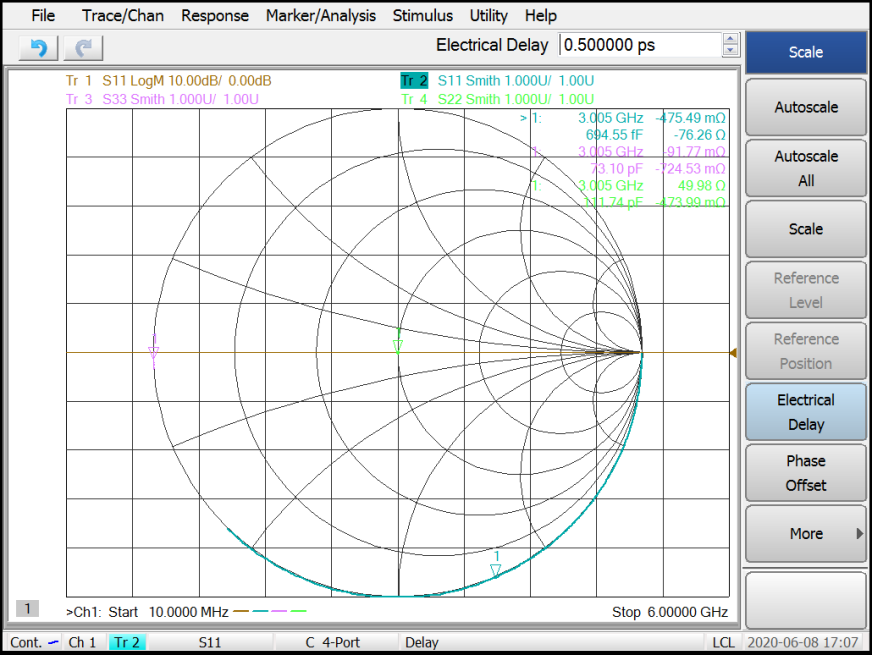
\includegraphics[width=\textwidth]{2_3_2}
  \caption{Smithdiagramm der S11-Messung, im Trace 2 ist ein Kapazitiver anteil
    bei offenem Abschluss erkennbar}
  \label{fig:2_3_2}
\end{figure}

\begin{figure}[h]
  \begin{center}
  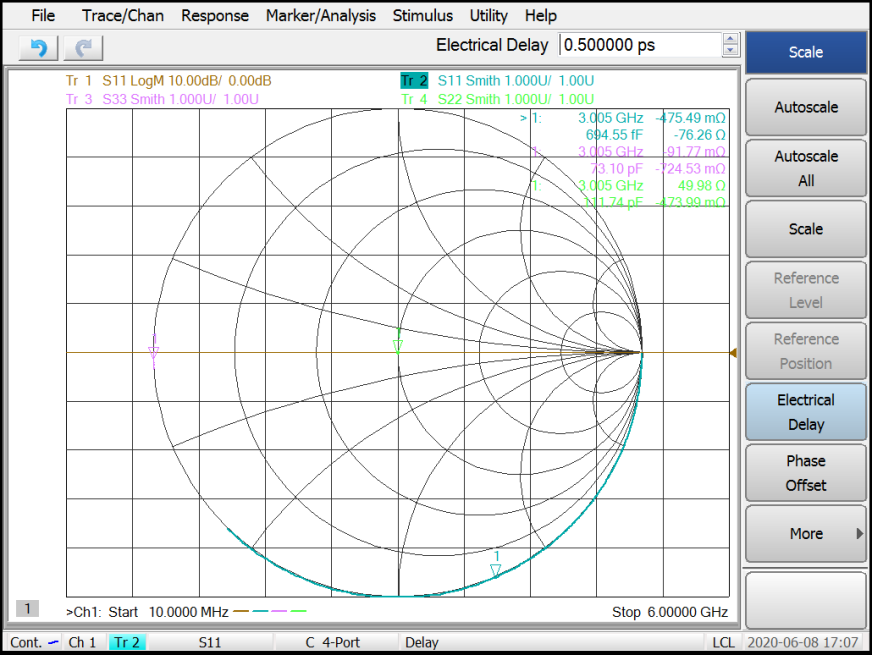
\includegraphics[width=0.618\textwidth]{2_3_2}
  \caption{Smithdiagramm der S11-Messung, mit Korrekturparameter, Türkis: Open,
    Grün: Load, Pink: Short}
  \label{fig:2_3_1}
  \end{center}
\end{figure}

\begin{figure}[h]
  \begin{center}
  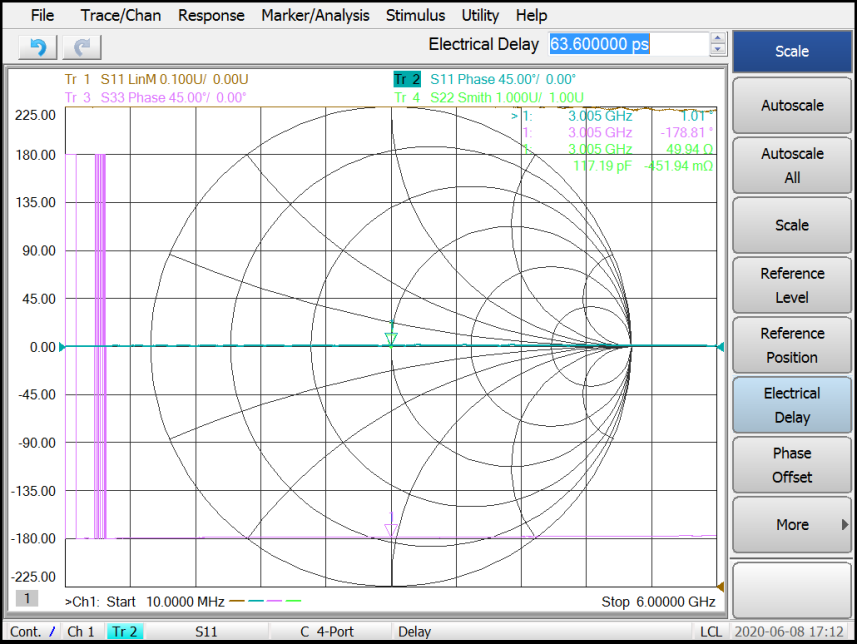
\includegraphics[width=0.618\textwidth]{phase}
  \caption{Phasen der S11-Messung, Farben entsprechen Abb. \ref{fig:2_3_1}}
  \label{fig:phase_2_3}
  \end{center}
\end{figure}

Mithilfe eines mechanischen Standards wurde das DUT, ein Koaxialkabel,
jeweils mit Short, Open und Load abgeschlossen und der S11-Parameter mit dem
Netzwerkanalysator als Frequenzgang bestimmt. Vorher musste noch der kapazitive
Anteil des S11 mithilfe eines \emph{Electrical Delays} in der Software des
Netzwerkanalysators kompensiert werden (Abb. \ref{fig:2_3_2}).

Daraufhin wurde
die S11-Parameter Leitung bei den entsprechenden Abschlüssen gemessen und unter
Umständen mit einem Electrical Delay beaufschlagt. Im Ergebniss erkennt man die
S11-Positionen im Smithdiagramm bei Short am linken Rand mit Phase $-180 \, \si{\degree}$ (0 auf der reelen
Achse), also Totalreflexion, bei Open am rechten Rand mit Phase $0 \, \si{\degree}$ ($\infty$ auf der reelen
Achse), auch Totalreflexion, und bei Load in der Mitte ($1$ auf der reelen
Achse). Das Smithdiagramm zeigt die erwarteten Ergebnisse (Abb. \ref{fig:2_3_1}).

Über der Frequenz
waren die Reflexionsfaktoren bei Short sowie Open entsprechend $0 \,
\si{\deci\bel}$ und bei Load (Anpassung) bei einem sehr geringen Wert, was
ebenfalls zu erwarten war.


\subsection{Dämpfungsglied}
\begin{figure}[h]
  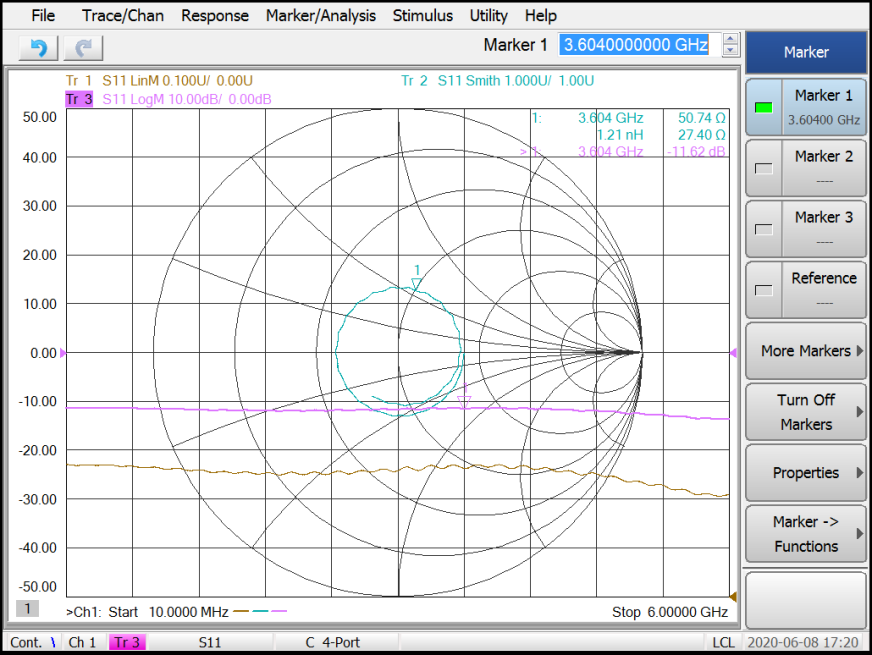
\includegraphics[width=\textwidth]{2_4}
  \caption{Smithdiagramm der S11-Messung des Dämpfungsgliedes}
  \label{fig:2_4_smith}
\end{figure}

Im Versuch wurde zuerst der S11-Parameter eines Dämpfungsgliedes bestimmt. Das
Ergebnis im Smith-Format ist in Abb. \ref{fig:2_4_smith} zu sehen.

Der Reflexionsfaktor zeigt eine Frequenzabhängigkeit, welche sich im
Smithdiagramm durch den kreisförmigen Verlauf (Abb. \ref{fig:2_4_smith} türkis)
äußert.

\begin{figure}[h]
  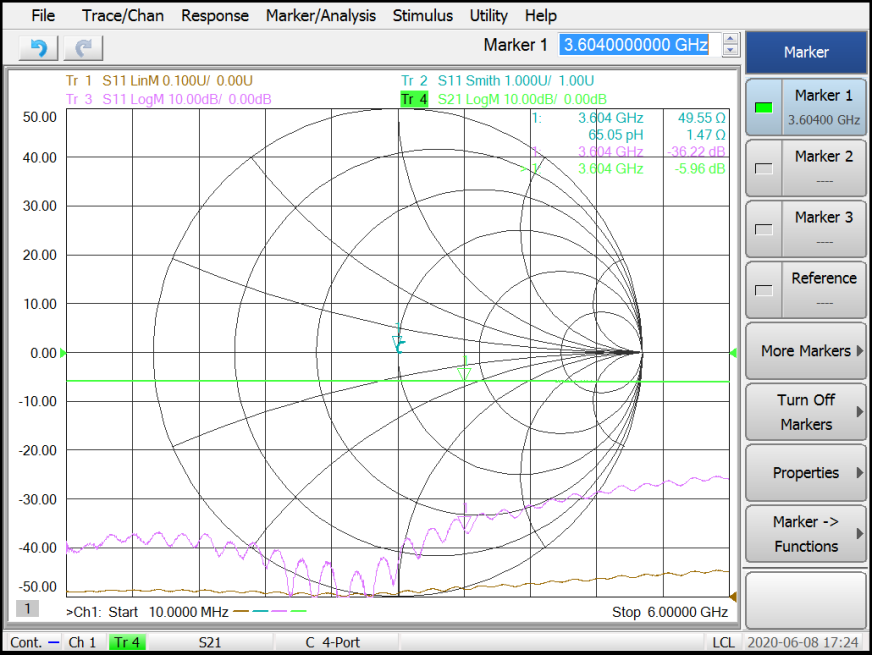
\includegraphics[width=\textwidth]{2_4_c_einfuge}
  \caption{Messung der Einfügedämpfung des Dämpfungsgliedes (grün)}
  \label{fig:2_4_einfuge}
\end{figure}

Mit einer Messung der Transmission/Einfügedämpfung und dafür notwendiger vorheriger Verbindung
eines zweiten Ports ergab sich die Übertragungsfunktion des Dämpfungsgliedes.
Die Einfügedämpfung ist in Abb. \ref{fig:2_4_einfuge} zu sehen. Man erkennt die konstante
Dämpfung von etwa $-5.96 \, \si{\deci\bel}$ über den betrachteten Frequenzbereich.

\begin{figure}[h]
  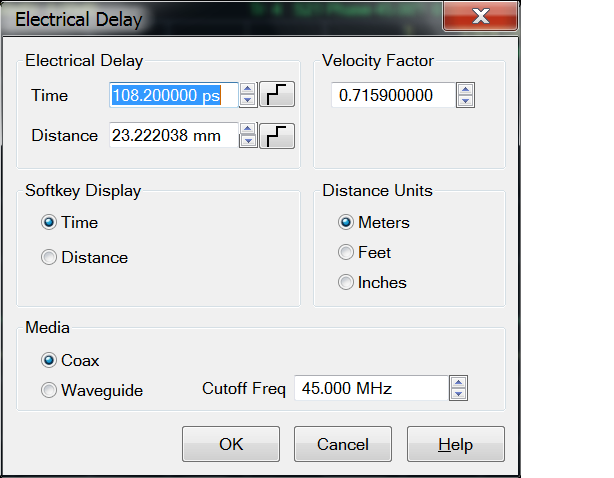
\includegraphics[width=\textwidth]{Elektrische_lange}
  \caption{Bestimmung der physikalischen Länge mithilfe des Electrical Delays}
  \label{fig:laenge1}
\end{figure}

Die ausschalggebende Größe für die Bestimmung der elektrischen bzw.
physikalischen Länge ist die Phase des Dämpfungsgliedes. Diese wurde gemessen
und das Electrical Delay angepasst, bis der Phasenverlauf inetwa $0
\si{\degree}$ im Frequenzgang entspricht. Über den voreingestellten
Verkürzungsfaktor im Fenster \emph{Electrical Delay} errechnete das Programm die
physikalische Länge des DUT (Abb. \ref{fig:laenge1}, \textit{Distance}), welche
mit der Messung durch ein Lineal positiv überprüft werden konnte.




\subsection{Untersuchung an Koaxialkabeln}
Im Versuch wurden S11 Messungen von einem BNC- und einem SMA-Kabel durchgeführt sowie deren
Verkürzungsfaktor bestimmt.

\begin{figure}[h]
  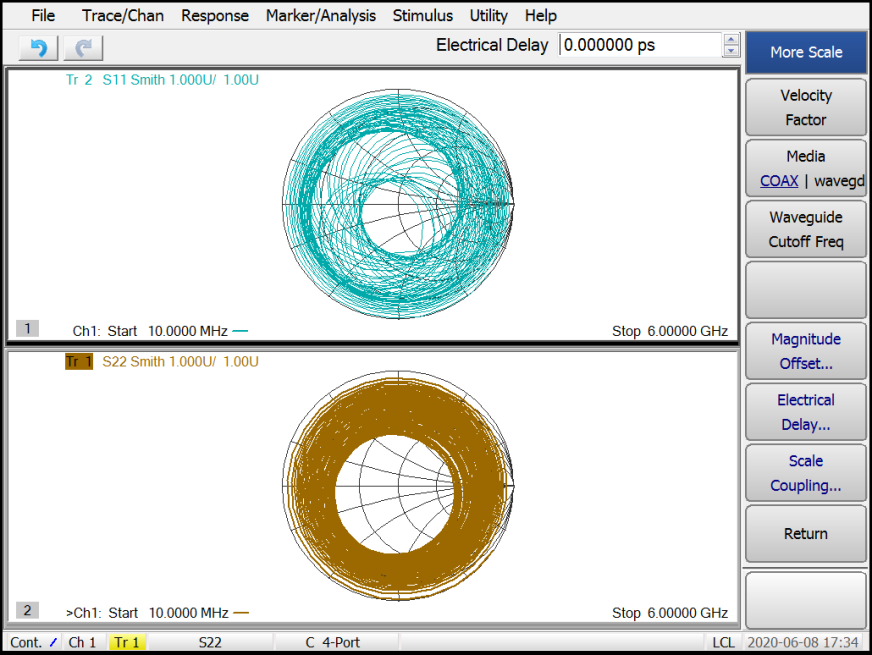
\includegraphics[width=\textwidth]{2_5}
  \caption{S11/S22 Messung von BNC (S11, blau) und SMA (S22, braun) im
    Smithdiagramm, offener Abschluss}
  \label{fig:circly}
\end{figure}

\begin{figure}[h]
  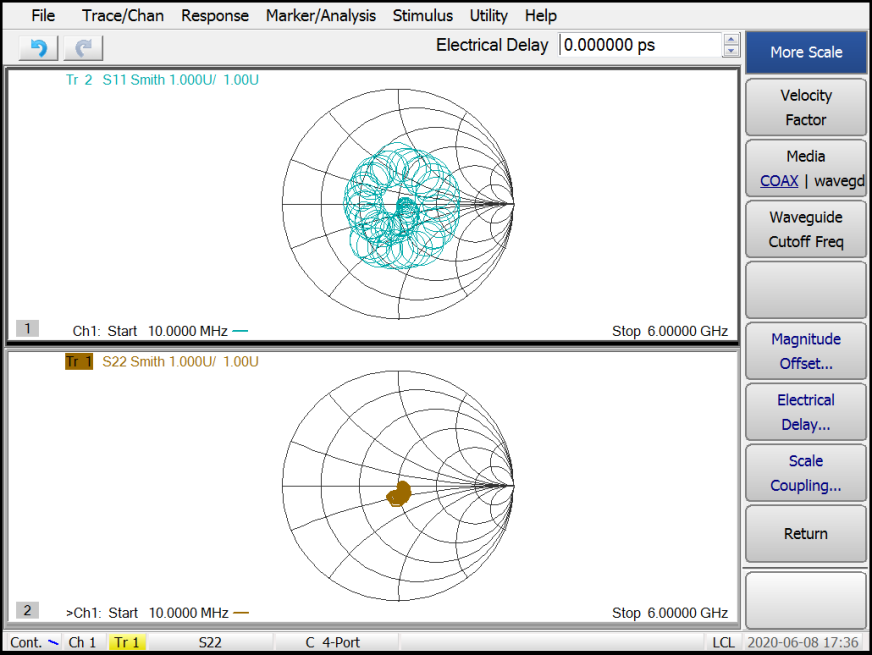
\includegraphics[width=\textwidth]{2_5_zusamme}
  \caption{S11/S22 Messung von BNC (S11, blau) und SMA (S22, braun) im
    Smithdiagramm, Abschluss}
  \label{fig:circly_load}
\end{figure}

Qualitativ kann aus dem Smithdiagramm Abb. \ref{fig:circly} erkannt werden, dass
der Reflexionsfaktor des BNC-Kabels deutlich frequenzabhängiger ist, als der des
SMA-Kabels.

Bei der Transmissionsmessung über S31 bzw. S42 wurde der zweite Port
verbunden und somit die Leitung abgeschlossen, die Auswirkung auf den
Reflexionsfaktor sieht man in Abb. \ref{fig:circly_load}. Das BNC-Kabel weist
auch hier noch einen sehr frequenzabhängigen und hohen Reflexionsfaktor im
gemssenen Frequenzbereich auf. Die Messung der Transmission ergab Abb.
\ref{fig:trans}. Auch bei der Transmission (Übertragungsfunktion) erkennt man
einen weniger linearen Verlauf des BNC-Kabels, was in Bezug auf die Güte einen
Nachteil gegenüber der SMA-Leitung darstell, was in Bezug auf die Güte einen
Nachteil gegenüber der SMA-Leitung darstelltt.

\begin{figure}[h]
  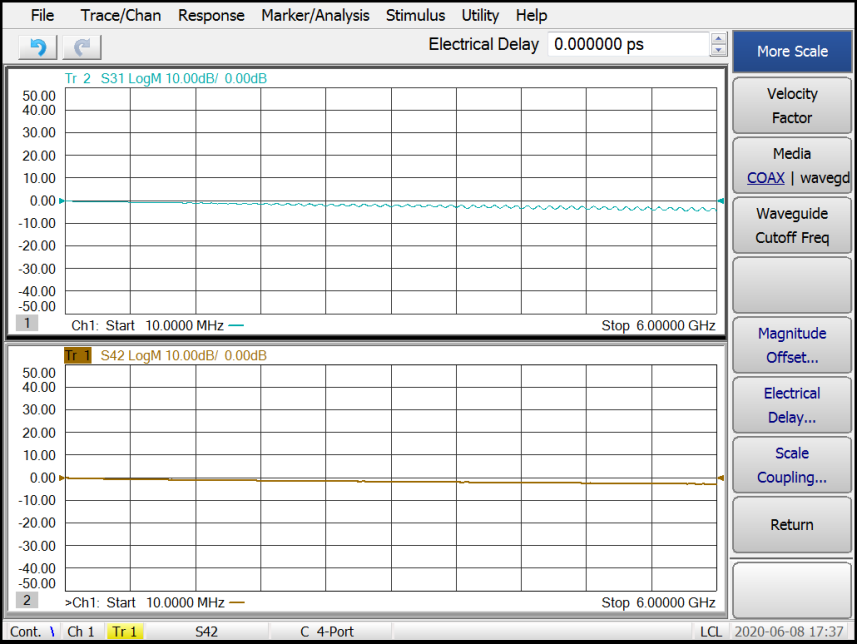
\includegraphics[width=\textwidth]{2_5_trans}
  \caption{Transmissionmessung von SMA und BNC} 
  \label{fig:circly_load}
\end{figure}

\begin{figure}[h]
  \begin{center}
  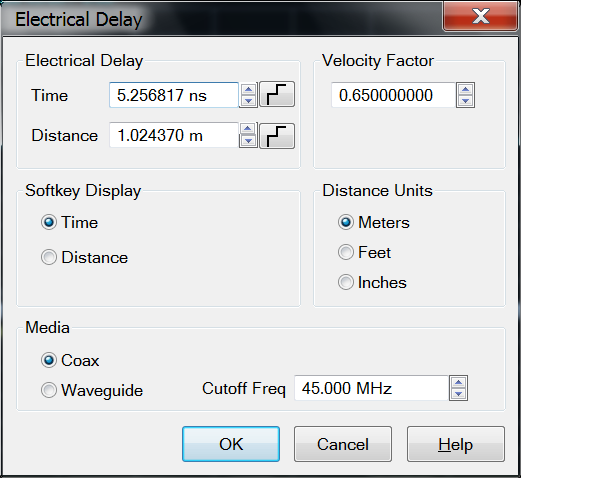
\includegraphics[width=0.618\textwidth]{BNC_lange}
  \end{center}
  \caption{Bestimmung des BNC-Verkürzungsfaktors}
  \label{fig:BNC_lange}
\end{figure}
\begin{figure}[h]
  \begin{center}
  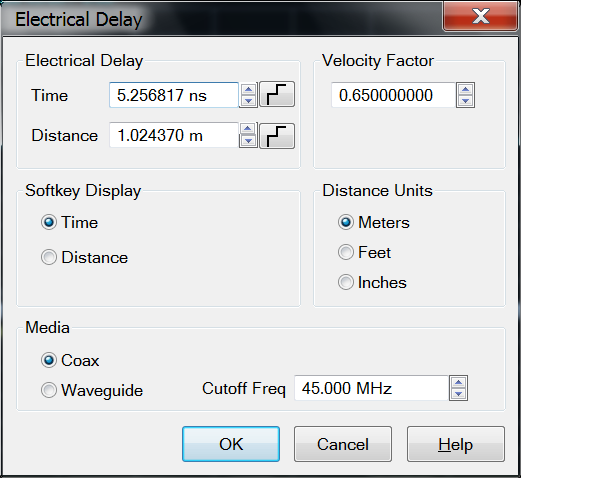
\includegraphics[width=0.618\textwidth]{BNC_lange}
  \end{center}
  \caption{Bestimmung des SMA-Verkürzungsfaktors}
  \label{fig:SMA_lange}
\end{figure}

Die Bestimmung des Verkürzungsfaktors der Leitungen erfolgte mithilfe der
Softwarelösung des Netzwerkanalysators, ähnlich zu der Methode aus der
vorherigen Aufgabe beim Dämpfungsglied. Das Electrical Delay wurde solange
angepasst, bis die Phase den Wert $0$ annahm. Da die Länge der Leitungen
bekannt war (jeweils $1 \, \si{\meter}$) konnte das Ergebnis für den
Verkürzungsfaktor überprüft werden.








\end{document}
